\newpage
\section{Tuning distance-dependency}

Stepping away, we 




Maybe simplicity of the model makes stuff wrong. Tune to Perin
distance profile.

Let 

In their study, \textcite{Perin2011} heavily rely on a
distance-dependent 


Here we introduce anisotropic networks tuned to reflect a given
distance-dependent connection profile $C(x)$. We are faced with the
following problem: Given $C(x):[0,\sqrt{2}) \to [0,1]$, find
$w:[0,\sqrt{2}) \to [0,\infty)$ such that the probability to have a
connection from $v_1$ to $v_2$ for arbitrary vertices $v_1 \neq v_2$ in an
anisotropic graph $G(n,w)$ with distance $\mathrm{d}(v_1,v_2) = x$ is
$C(x)$. The problem is in general highly complex, when nothing can be
assumed about $C(x)$. We find an approximate solution to the problem
regarding the following geometric relation:

\begin{figure}[htp]
  \centering
  \makebox{%
    \begin{overpic}[height=4.05cm]{%
        plots/bed7650b.pdf}
    \end{overpic}
  }%
  \caption{Computing connection probability $C(x)$ from non-constant $w(x)$}
  \label{fig:dpp_wc}
\end{figure}

From \autoref{fig:dpp_wc} we have the relation  
\begin{equation}
C\left(\sqrt{x^2+w^2(x)}\right) = \frac{1}{\pi} \operatorname{arctan}
\frac{w(x)}{x}. \label{eq:geo_rel}
\end{equation} 
In order to solve for $w(x)$ we first consider a linear approximation,
expanding
\[C\left(\sqrt{x^2+w^2(x)}\right) \approx C(x) + \left(\sqrt{x^2+w^2(x)} -
x\right) C'(x).\]

The resulting transcendental equation
\[C(x) + \left(\sqrt{x^2+w^2(x)} -
x\right) C'(x) = \frac{1}{\pi} \operatorname{arctan}
\frac{w(x)}{x}\]
is however still too complex in the context of this work. Instead we
propose the approximation $\sqrt{x^2 + w^2(x)} \approx  x$, which
inserting into \ref{eq:geo_rel} yiels
\begin{equation}
C(x) \approx \frac{1}{\pi} \operatorname{arctan} \label{eq:tanapprox}
\frac{w(x)}{x}.
\end{equation}

Under the assumption that $C(x)<\frac{1}{2}$ for all $x$ we obtain the
identity
\begin{equation}
  w(x) = x \tan\left( \pi\, C(x) \right), \label{eq:xtan}
\end{equation} 
being aware that it only holds as well as
approximation~\ref{eq:tanapprox} does. 

Here we use relation~\ref{eq:xtan} to generate anisotropic networks
reflecting the dis\-tance-de\-pendent connectivity profile as found by
\textcite{Perin2011}. For this we finally need to adjust the before
arbitrarily determined side length of the network's surface. Perin et
al.~mapped connectivity in layer 5 of the rat's somatosensory cortex
up to a distance of $\SI{300}{\micro\meter}$. Using this reported
distance connectivity to generate anisotropic networks via
\ref{eq:xtan}, the chosen side length $s$ determines the networks
overall connectivity (\autoref{fig:determine_side_length} A). We
determine $s = \SI{296}{\micro\meter}$ to match the overall connection
probability of $p = 0.116$ as used before and reported by Song et
al.~(\autoref{fig:determine_side_length} B). The obtained value for
$s$ is consistent with the slice thickness of \SI{300}{\micro\meter}
used in Perin et al.'s experiment.


\begin{figure}[htp]
  \centering
  \makebox{%
    \begin{overpic}[height=4.05cm]{%
        plots/6154302f.pdf}
      \put(85.5,57.0){\small\textbf{A}}
      %\put(12,5){\small\textbf{A}}
    \end{overpic}
    \hfill
    \begin{overpic}[height=4cm]{%
        plots/ef0e785d.pdf}
      \put(88.5,58.2){\small\textbf{B}}
    \end{overpic}
  }%
  
  \caption{\textbf{Network side length adjusted to match overall
      connection probability} 
    \textbf{A-B)} Side length of the network's surface determines the
    connection probability, in B) length $s$ is matched to $p =
    0.116$, as reported by \textcite{Song2005}. \textbf{C)} Resulting
    axon width function $w(x)$ from tuning to distance-dependent
    connection profile as reported by \textcite{Perin2011}, see also
    \autoref{fig:perin_profiles}. Note that $x \gg w(x)$ for most $x$,
    justifying the approximation~\ref{eq:tanapprox}. \textbf{D)}
    Showing for a single neuron (star) connected (red) and unconnected
    (gray) neurons in the tuned anisotropic network, revealing
    characteristic new axon shape.}
  \label{fig:determine_side_length}
\end{figure}



Having determined the neotwork's side length $s$, we're extending the
quiver of generated sample networks for the numerical analysis once
more by the \enquote{tuned anisotropic graphs} \index{tuned
  anisotropic networks}, in which the axon width $w(x)$ was determined
such that the networks reflect Perin's connectivity profile. Analyzing
the obtained axon width function we note that $x \gg w(x)$ holds for
most $x$, justifying the approximation
\[\sqrt{x^2 + w^2(x)} \approx
x\] \textit{a posteriori} (\autoref{fig:perin_axwidth}). From the 25
generated networks overall connection probability is extracted as $p
= 0.1160 \pm 0.0006$ (SEM), as expected from the choice of $s$ (\smtcite{f11dca65}).



% This approximation holds well as long as $x \gg w(x)$. Using the
% relation to tune the axon width to produce anisotropic networks with a
% distance-dependency as reported by Perin et al., we find that for all $x$ is
% strictly greater than $w(x)$  %(\autoref{fig:perin_axwidh


\begin{figure}[htp]
  \centering
  \hspace{0.05cm}
  \begin{overpic}[width=0.6\textwidth]{%
      /users/hoffmann/research/tanfit_width_test.pdf}
          \put(69.4,51.5){\small\textbf{A}}
  \end{overpic}
  \hfill
  \begin{overpic}[width=0.35\textwidth]{%
      /users/hoffmann/research/connected_test.pdf}
    \put(81,86){%
      \fboxsep=2pt\colorbox{white}{\small\textbf{B}}
    }
  \end{overpic}

  \vspace{-0.15cm}

  \caption{\textbf{Anisotropic network model with tuned axon width
      $\mathbf{w(x)}$} \textbf{A-B)} Side length of the network's
    surface determines the connection probability, in B) length $s$ is
    matched to $p = 0.116$, as reported by
    \textcite{Song2005}. \textbf{C)} Resulting axon width function
    $w(x)$ from tuning to distance-dependent connection profile as
    reported by \textcite{Perin2011}, see also
    \autoref{fig:perin_profiles}. Note that $x \gg w(x)$ for most $x$,
    justifying the approximation~\ref{eq:tanapprox}. \textbf{D)}
    Showing for a single neuron (star) connected (red) and unconnected
    (gray) neurons in the tuned anisotropic network, revealing
    characteristic new axon shape.}
  \label{fig:perin_axwidth}
\end{figure}


% \begin{figure}[htp]
%   \centering
%   \makebox{%
%     \begin{overpic}[height=4.05cm]{%
%         plots/6154302f.pdf}
%       \put(85.5,57.0){\small\textbf{A}}
%       %\put(12,5){\small\textbf{A}}
%     \end{overpic}
%     \hfill
%     \begin{overpic}[height=4cm]{%
%         plots/ef0e785d.pdf}
%       \put(88.5,58.2){\small\textbf{B}}
%     \end{overpic}
%   }%
%   \vfill
%   \hspace{0.05cm}
%   \begin{overpic}[width=0.6\textwidth]{%
%       /users/hoffmann/research/tanfit_width_test.pdf}
%           \put(69.4,51.5){\small\textbf{C}}
%   \end{overpic}
%   \hfill
%   \begin{overpic}[width=0.35\textwidth]{%
%       /users/hoffmann/research/connected_test.pdf}
%     \put(81,86){%
%       \fboxsep=2pt\colorbox{white}{\small\textbf{D}}
%     }
%   \end{overpic}

%   \vspace{-0.15cm}

%   \caption{\textbf{Anisotropic network model with tuned axon width
%       $\mathbf{w(x)}$} \textbf{A-B)} Side length of the network's
%     surface determines the connection probability, in B) length $s$ is
%     matched to $p = 0.116$, as reported by
%     \textcite{Song2005}. \textbf{C)} Resulting axon width function
%     $w(x)$ from tuning to distance-dependent connection profile as
%     reported by \textcite{Perin2011}, see also
%     \autoref{fig:perin_profiles}. Note that $x \gg w(x)$ for most $x$,
%     justifying the approximation~\ref{eq:tanapprox}. \textbf{D)}
%     Showing for a single neuron (star) connected (red) and unconnected
%     (gray) neurons in the tuned anisotropic network, revealing
%     characteristic new axon shape.}
%   \label{fig:determine_side_length}
% \end{figure}












\begin{figure}[htp]
  \centering
  \makebox{%
    \begin{overpic}[width=0.5\textwidth]{%
        plots/875505b0_overall.pdf}
      \put(28,19){\small\textbf{A}}
    \end{overpic}
    \hfill
    \begin{overpic}[width=0.5\textwidth]{%
        plots/875505b0_single.pdf}
      \put(28,19){\small\textbf{B}}
    \end{overpic}
  }%
  \vspace{-0.6cm}
  \makebox{%
    \begin{overpic}[width=0.5\textwidth]{%
        plots/875505b0_recip.pdf}
       \put(28,19){\small\textbf{C}}
    \end{overpic}
    \vspace{-1cm}
    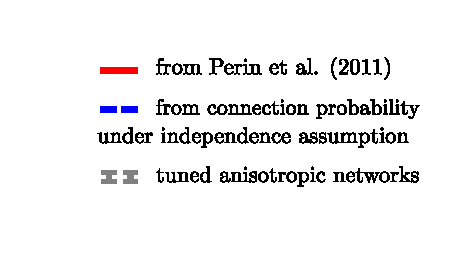
\includegraphics[width=0.5\textwidth]{%
      img/tuned_legend.pdf}   
  }%
  \vspace{-0.15cm}
  \caption{\textbf{Overrepresentation of reciprocal connections
      independent of } Comparison of occurrences of one- and
    bidirectionally connected neuron pairs in (gray) with profiles
    found by \textcite{Perin2011} (red), shows that overrepresentation of
    bidirectional pairs is distance-independent and not connected to
    anisotropy.  \textbf{A)} Overall connection probability in the
    adapted anisotropic networks was successfully tuned to reflect
    connection probability found by Perin et al. \textbf{B)-C)}
    Probabilities for a random neuron pair to display , 
    (\smtcite{875505b0})} %?? fix width issue!!
  \label{fig:perin_profiles}
\end{figure}



%%% Local Variables: 
%%% mode: latex
%%% TeX-master: "../dplths_document"
%%% End: 


% \begin{figure}[htp]
%   \centering
%     \begin{minipage}{.45\textwidth}

%         \begin{overpic}[width=\textwidth]{%
%             plots/6154302f.pdf}
%           \put(85.5,57.5){\small\textbf{A}}
%           % \put(12,5){\small\textbf{A}}
%         \end{overpic}
%         \vfill
%         \begin{overpic}[width=\textwidth]{%
%             plots/ef0e785d.pdf}
%           \put(90.5,58.2){\small\textbf{B}}
%         \end{overpic}

%       \end{minipage}
%       \hfill
%       \begin{minipage}{.45\textwidth}

%         \begin{overpic}[width=0.85\textwidth]{%
%             plots/bed7650b.pdf}
%         \end{overpic}
%        \vfill

%         \begin{overpic}[width=0.85\textwidth]{%
%             /users/hoffmann/research/connected_test.pdf}
%           % \put(90.5,58.2){\small\textbf{B}}
%         \end{overpic}
 
        
%       \end{minipage}
      
%   \vspace{-0.15cm}
%   \caption{ (\smtcite{6154302f}, \smtcite{ef0e785d})} %?? fix width issue!!
%   \label{fig:determine_side_length}
% \end{figure}


% \begin{figure}[htp]
%   \centering
%   \makebox{%
%     % \begin{overpic}[height=4.05cm]{%
%     %     plots/6154302f.pdf}
%     %   \put(85.5,57.5){\small\textbf{A}}
%     %   %\put(12,5){\small\textbf{A}}
%     % \end{overpic}
%     % \hfill
%     \begin{overpic}[height=4cm]{%
%         /users/hoffmann/research/connected_test.pdf}
%       % \put(90.5,58.2){\small\textbf{B}}
%     \end{overpic}
%   }%
%   \vspace{-0.15cm}
%   \caption{ (\smtcite{6154302f}, \smtcite{ef0e785d})} %?? fix width issue!!
%   \label{fig:tuned_width}
% \end{figure}